\documentclass[10pt,a4paper]{article}
\usepackage[utf8]{inputenc}
\usepackage[german]{babel}
\usepackage{amsmath}
\usepackage{amsfonts}
\usepackage{amssymb}
\usepackage{mhchem}
\usepackage{siunitx}
\usepackage{multirow}
\usepackage[left=2cm,right=2cm,top=2cm,bottom=2cm]{geometry}
\usepackage{wrapfig}
\usepackage{graphicx}
\usepackage[outdir=./]{epstopdf}
\usepackage{caption}
\usepackage[colorlinks]{hyperref}


\author{Christian Bespin \and Christopher Deutsch}
\title{Übungsblatt 3: Numerische Methoden der Physik}
\begin{document}
\maketitle

\setcounter{section}{1}

\section{Treibhauseffekt}

\subsection{Physikalischer Hintergrund}
Der Treibhauseffekt beschreibt den Einfluss der Atmosphäre und der in ihr
auftretenden Gase auf die Temperatur der Erde. Während die Sonnenstrahlung die
Atmosphäre zu großen Teilen durchdringt, wird die von der Erde emittierte
infrarote Strahlung von den Gasen der Atmosphäre absorbiert (vorallem durch Wasserdampf
aber auch durch Spurengase wie \ce{CO2}), was zu einer Erwärmung des Klimas führt.

Zur Erklärung des Treibhauseffektes wird ein Modell grauer und schwarzer Körper
im thermischen Gleichgewicht verwendet. Wir beschreiben die Erde als schwarzen
Strahler mit Emissions-/Absorptionsgrad $\epsilon_E = \alpha_E = 1$. Die Sonne 
wird durch einen grauen Strahler der Temperatur $T_S$ mit Emissionsgrad
$\epsilon_S = \text{konst.}$ ersetzt.
Auch die Atmosphäre wird als grauer Strahler modelliert. Dieser habe die
Temperatur $\tau$ und den Emissionsgrad $\epsilon(\tau)$. 
Das Kirchhoff'sche Strahlungsgesetz besagt, dass der Emissionsgrad $\epsilon$ eines
grauen Körpers gleich seinem Absorptionsgrad $\alpha$ ist. Demnach hat die
Atmosphäre für Strahlung der Temperatur $T$ den Absorptionsgrad $\alpha(T) = \epsilon(T)$.

\begin{wrapfigure}[14]{R}[1pt]{0.47\textwidth}
\centering
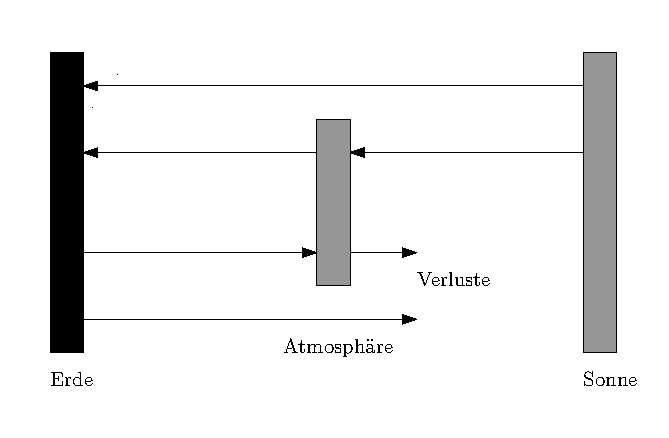
\includegraphics[width=0.45\textwidth]{./figures/strahlungsgleichgewicht.eps}
\caption{Strahlungsgleichgewicht}
\label{fig:strahlungsgleichgewicht}
\end{wrapfigure}
Ein Körper ist im thermischen Gleichgewicht, wenn seine abgestrahlte Leistung
gleich seiner absorbierten Leistung ist. Diese wird durch das Stefan-Boltzmann-Gesetz
$P \propto \epsilon T^4$ beschrieben. Die Gleichgewichtsbedingung für die Atmosphäre ist:
\begin{align}
	2\epsilon(\tau)\tau^4 &= \alpha(T_S) \epsilon_S T_S^4 + \alpha(T_E) \epsilon_E T_E^4 \notag \\ &=\epsilon(T_S) \epsilon_S T_S^4 + \epsilon(T_E) T_E^4
\end{align}
Dabei wurde die Proportionalitätskonstante aus der Gleichung heraus gekürzt.
Der Term auf der linken Seite beschreibt die Abstrahlung der Atmosphäre, wobei
Faktor $2$ die Abstrahlung sowohl zur Erde als auch zur Sonne beschreibt.
Die rechte Seite beschreibt die Absorption, dabei wurde erst im letzten
Umformungsschritt $\epsilon_E = 1$ und das Kirchhoff'sche Strahlungsgesetz verwendet,
um den Unterschied zwischen der Absorption der Atmosphäre und des Emissionsgrades von
Sonne/Erde deutlich zu machen.
Analog dazu erhält man zwei weitere Gleichgewichtsbedingungen, aus denen man
$\tau$ eliminieren kann und eine Bestimmungsgleichung für die Temperatur $T_E$
der Erde im Gleichgewicht erhält:
\begin{align}
\left[2-\epsilon(T_E)\right]T_E^4=\epsilon_S\left[2-\epsilon(T_S)\right]T_S^4
\label{eqn:gleichgewicht}
\end{align}
Der Emissionsgrad ergibt sich aus dem Verhältnis von spezifischer Ausstrahlung des Körpers in den Halbraum zur spezifischen Ausstrahlung eines schwarzen Körpers derselben Temperatur (Stefan-Boltzmann-Gesetz). 

Die spezifische Ausstrahlung erhält man durch Integration der spektralen Energiedichte (Planck'sches Gesetz) über alle Frequenzen $\nu$. Dabei muss bei der spezifischen Ausstrahlung der Atmosphäre beachtet werden, dass die spektrale Energiedichte mit $1-f(\nu)$ gewichtet wird, was die Wahrscheinlichkeit darstellt, dass ein Photon von \ce{CO2} absorbiert wird.

Dementsprechend ist $f(\nu) = \exp\left(-N \sigma(\nu) \right)$ mit $N = \tilde{n} N_0$ die Wahrscheinlichkeit, dass ein Photon die Atmosphäre durchdringen kann. Dabei ist $N_0 = \num{7.3e25}\,\si{\per\metre^2}$ die aktuelle Anzahl von \ce{CO2} Molekülen in einer Luftsäule mit $\num{1}\,\si{\metre^2}$ Grundfläche. Für den Wirkungsquerschnitt $\sigma(\nu)$ von \ce{CO2} wurde die Breit-Wigner-Formel mit Resonanzen bei $\nu_2 = \num{2.00e13}\, \si{\per\second}$ und $\nu_3 = \num{7.04e13}\, \si{\per\second}$ angenommen.


\subsection{Implementierung}
Im Wesentlichen besteht unser Programm aus zwei Teilen:
\begin{enumerate}
	\item die benötigten numerischen Methoden zum Lösen der nichtlinearen Gleichung (\ref{eqn:gleichgewicht}), also Integration und numerisches Lösen von Gleichungen
	\item die konkrete Implementierung des physikalischen Problems
\end{enumerate}
Wir haben uns bemüht, diese Teile im Quellcode strikt zu trennen, um Übersichtlichkeit zu gewährleisten. Die numerischen Methoden finden sich in dem Modul \texttt{numerik\_bespin\_deutsch\_mathfunctions} und die Lösung des physikalischen Problems in der Hauptquelldatei \texttt{numerik\_bespin\_deutsch\_3.c}

\subsubsection{Nullstellenberechnung mit Bisektion}

Ein Verfahren, um numerisch Nullstellen zu bestimmen, ist das Iterationsverfahren der Bisektion. Dabei wird vorausgesetzt, dass die Funktion auf dem relevanten Intervall $[a,b]$ stetig ist und dort einen Vorzeichenwechsel hat. Dann folgt aus dem Zwischenwertsatz, dass dort garantiert eine Nullstelle liegt. Die Bisektion halbiert zunächst das zu betrachtende Intervall und prüft, ob zwischen den Grenzen der Teilintervalle ein Vorzeichenwechsel in den Funktionswerten vorliegt. Da die Funktion nach Voraussetzung nur einen Vorzeichenwechsel auf dem ganzen Intervall hatte, tritt in einem der Teilintervalle kein Vorzeichenwechsel auf und dieses wird im Folgenden vernachlässigt. Bei dem nächsten Schleifendurchlauf wird dieses Verfahren auf das verbleibende Teilintervall angewendet. Das Intervall, auf dem der Vorzeichenwechsel stattfindet, wird so immer weiter eingeschränkt, bis es eine gewünschte vorgegebene Genauigkeit erreicht (Intervallbreite $<\epsilon$). 
Wir verwenden die Bisektion hier, da im Gegensatz zum Newtonverfahren keine Ableitungen der Funktion  berechnet werden müssen. Bei der hier vorliegenden Funktion ist die Ableitung nur numerisch bestimmbar, was den Rechenaufwand erheblich beeinträchtigen würde.

\subsubsection{Numerische Integration mit rekursivem Simpson-Verfahren}
\label{sssec:integration}

Die Simpson-Methode nähert das Integral einer Funktion $f$ auf dem Intervall $[x_0,x_2]$ durch das Integral des Interpolationspolynoms mit den Stützstellen $x_0$, $x_1$ und $x_2$, wobei $x_1$ gerade das Intervall halbiert. Die Auswertung der Näherung ist:
\begin{align}
  \int_{x_0}^{x_2} f(x) \, \mathrm{d}x \approx \frac{h}{6} \left( f(x_0) + 4 f(x_1) + f(x_2) \right) \quad \text{mit } h = x_2 - x_0
\end{align}
Man kann die Näherung des Integrals verbessern, indem man das Intervall halbiert und schließlich auf den Teilintervallen erneut die Simpson-Methode anwendet. Dies kann je nach Präzisionsbedarf beliebig oft wiederholt werden.

Wir haben uns für die Implementierung der adaptiven Simpson-Methode entschieden, bei der das Integral rekursiv berechnet wird. Dazu wird zunächst eine erste Näherung des Integrals auf dem Gesamtintervall durchgeführt. Dann wird das zu integrierende Intervall halbiert und anschließend werden diese Teilintervalle mit der Simpson-Methode ausgewertet. Sollte die Differenz der Summe der integrierten Teilintervalle und des Gesamtintervalls eine Grenze $\epsilon$ überschreiten, wird das Verfahren auf jedem der Teilintervalle wiederholt. Da bei der Rekursion die Intervalle halbiert werden, muss auch mit jedem Schritt die Grenze $\epsilon$ halbiert werden, um eine sinnvolle Fehlereinschätzung zu gewährleisten. In \cite{lyness} wird gezeigt, dass $\epsilon / 15$ ein guter Schätzer für den absoluten Fehler der Näherung ist.

Der Vorteil einer rekursiven Umsetzung ist, dass sich der adaptive Mechanismus leicht implementieren lässt, da sich jedes Teilintervall unabhängig betrachten lässt. Dabei ist die Idee, dass man eine sehr feine Intervallteilung in Bereichen starker und eine sehr grobe in Bereichen minimaler Änderung des Integranden vornimmt. Für die Implementierung ist wichtig, dass bereits berechnete Funktionswerte rekursiv weitergegeben werden, um die Anzahl der Funktionsauswertungen zu minimieren.


\subsubsection{Lösung des physikalischen Problems}

Zur Berechnung der Temperatur der Erde im thermischen Gleichgewicht formen wir Gleichung (\ref{eqn:gleichgewicht}) in ein Nullstellenproblem um, welches mithilfe von Bisektion gelöst werden kann.
\begin{align}
	\left[2-\epsilon(T_E)\right]T_E^4 - \epsilon_S\left[2-\epsilon(T_S)\right]T_S^4 = 0
	\label{eq:nullstellenproblem}
\end{align}
Dies wurde in der Funktion \texttt{equilibrium\_eqn} umgesetzt. Zur numerischen Lösung dieser Gleichung muss die Emissivität der Atmosphäre berechnet werden. Diese hängt unter anderem von der integrierten spektralen Energiedichte $Z(T)$ ab, welche analytisch berechnet wird:
\begin{align}
	Z(T) = \frac{8}{15} \frac{\pi^5 \, k_B^4 \, T^4}{c^3 \, h^3}
\end{align}
Außerdem von dem Integral:
\begin{align}
	\int_0^\infty \rho(\nu,T)[1 - f(\nu)] \, \mathrm{d}\nu
\end{align}
welches mit der in Abschnitt \ref{sssec:integration} erklärten Methode berechnet wird.

Die Integration soll im Folgenden näher erläutert werden. Zunächst ist eine uneigentliche numerische Integration über ein Intervall unendlicher Länge nicht möglich. Dies ist in unserem Fall nicht nötig, da der Integrand nur auf einem endlichen Intervall signifikant von Null verschieden ist. Für unsere Berechnung interessant ist das Verhalten des Integranden für $T = \num{5750}\,\si{\kelvin}$ (Temperatur der Sonne), sowie $T = \num{300}\,\si{\kelvin}$ (in diesem Bereich erwarten wir die Gleichgewichtstemperatur der Erde) für $\num{0.1} < \tilde{n} < \num{100}$, wobei die obere Grenze sehr großzügig gewählt wurde. Aus den Abbildungen \ref{fig:integrand300} und \ref{fig:integrand5750} folgern wir, dass man $[10^{13}\,\si{\per\second},10^{15}\,\si{\per\second}]$ als sinnvolle Integrationsgrenzen für $T = \num{5750}\,\si{\kelvin}$ und $[10^{12}\,\si{\per\second}, 10^{14}\,\si{\per\second}]$ für $T = \num{300}\,\si{\kelvin}$ wählen kann. Darüber hinaus erwarten wir einen Wert des Integrals in der Größenordnung $10^{-6}\,\si{\joule\per\metre^3}$, weshalb die Abbruchbedingung der Integration (vgl. \ref{sssec:integration}) $\epsilon = 10^{-11}\,\si{\joule\per\metre^3}$ gewählt wurde, was einem absoluten Fehler von $\epsilon / 15 \approx 10^{-12}\,\si{\joule\per\metre^3}$ entspricht. Die hier erwähnten Maßnahmen wurden in der Funktion \texttt{emissivity} implementiert.

\subsection{Physikalische Ergebnisse}
\label{ssec:physikalischeergebnisse}
\begin{figure}[htpb!]
\centering
% GNUPLOT: LaTeX picture with Postscript
\begingroup
  \makeatletter
  \providecommand\color[2][]{%
    \GenericError{(gnuplot) \space\space\space\@spaces}{%
      Package color not loaded in conjunction with
      terminal option `colourtext'%
    }{See the gnuplot documentation for explanation.%
    }{Either use 'blacktext' in gnuplot or load the package
      color.sty in LaTeX.}%
    \renewcommand\color[2][]{}%
  }%
  \providecommand\includegraphics[2][]{%
    \GenericError{(gnuplot) \space\space\space\@spaces}{%
      Package graphicx or graphics not loaded%
    }{See the gnuplot documentation for explanation.%
    }{The gnuplot epslatex terminal needs graphicx.sty or graphics.sty.}%
    \renewcommand\includegraphics[2][]{}%
  }%
  \providecommand\rotatebox[2]{#2}%
  \@ifundefined{ifGPcolor}{%
    \newif\ifGPcolor
    \GPcolortrue
  }{}%
  \@ifundefined{ifGPblacktext}{%
    \newif\ifGPblacktext
    \GPblacktextfalse
  }{}%
  % define a \g@addto@macro without @ in the name:
  \let\gplgaddtomacro\g@addto@macro
  % define empty templates for all commands taking text:
  \gdef\gplbacktext{}%
  \gdef\gplfronttext{}%
  \makeatother
  \ifGPblacktext
    % no textcolor at all
    \def\colorrgb#1{}%
    \def\colorgray#1{}%
  \else
    % gray or color?
    \ifGPcolor
      \def\colorrgb#1{\color[rgb]{#1}}%
      \def\colorgray#1{\color[gray]{#1}}%
      \expandafter\def\csname LTw\endcsname{\color{white}}%
      \expandafter\def\csname LTb\endcsname{\color{black}}%
      \expandafter\def\csname LTa\endcsname{\color{black}}%
      \expandafter\def\csname LT0\endcsname{\color[rgb]{1,0,0}}%
      \expandafter\def\csname LT1\endcsname{\color[rgb]{0,1,0}}%
      \expandafter\def\csname LT2\endcsname{\color[rgb]{0,0,1}}%
      \expandafter\def\csname LT3\endcsname{\color[rgb]{1,0,1}}%
      \expandafter\def\csname LT4\endcsname{\color[rgb]{0,1,1}}%
      \expandafter\def\csname LT5\endcsname{\color[rgb]{1,1,0}}%
      \expandafter\def\csname LT6\endcsname{\color[rgb]{0,0,0}}%
      \expandafter\def\csname LT7\endcsname{\color[rgb]{1,0.3,0}}%
      \expandafter\def\csname LT8\endcsname{\color[rgb]{0.5,0.5,0.5}}%
    \else
      % gray
      \def\colorrgb#1{\color{black}}%
      \def\colorgray#1{\color[gray]{#1}}%
      \expandafter\def\csname LTw\endcsname{\color{white}}%
      \expandafter\def\csname LTb\endcsname{\color{black}}%
      \expandafter\def\csname LTa\endcsname{\color{black}}%
      \expandafter\def\csname LT0\endcsname{\color{black}}%
      \expandafter\def\csname LT1\endcsname{\color{black}}%
      \expandafter\def\csname LT2\endcsname{\color{black}}%
      \expandafter\def\csname LT3\endcsname{\color{black}}%
      \expandafter\def\csname LT4\endcsname{\color{black}}%
      \expandafter\def\csname LT5\endcsname{\color{black}}%
      \expandafter\def\csname LT6\endcsname{\color{black}}%
      \expandafter\def\csname LT7\endcsname{\color{black}}%
      \expandafter\def\csname LT8\endcsname{\color{black}}%
    \fi
  \fi
  \setlength{\unitlength}{0.0500bp}%
  \begin{picture}(7200.00,4320.00)%
    \gplgaddtomacro\gplbacktext{%
      \csname LTb\endcsname%
      \put(814,704){\makebox(0,0)[r]{\strut{} 10}}%
      \put(814,1076){\makebox(0,0)[r]{\strut{} 15}}%
      \put(814,1449){\makebox(0,0)[r]{\strut{} 20}}%
      \put(814,1821){\makebox(0,0)[r]{\strut{} 25}}%
      \put(814,2193){\makebox(0,0)[r]{\strut{} 30}}%
      \put(814,2566){\makebox(0,0)[r]{\strut{} 35}}%
      \put(814,2938){\makebox(0,0)[r]{\strut{} 40}}%
      \put(814,3310){\makebox(0,0)[r]{\strut{} 45}}%
      \put(814,3683){\makebox(0,0)[r]{\strut{} 50}}%
      \put(814,4055){\makebox(0,0)[r]{\strut{} 55}}%
      \put(946,484){\makebox(0,0){\strut{} 0}}%
      \put(2117,484){\makebox(0,0){\strut{} 2}}%
      \put(3289,484){\makebox(0,0){\strut{} 4}}%
      \put(4460,484){\makebox(0,0){\strut{} 6}}%
      \put(5632,484){\makebox(0,0){\strut{} 8}}%
      \put(6803,484){\makebox(0,0){\strut{} 10}}%
      \put(176,2379){\rotatebox{-270}{\makebox(0,0){\strut{}$T_E$ [\si{\celsius}]}}}%
      \put(3874,154){\makebox(0,0){\strut{}$n$}}%
      \put(3874,3945){\makebox(0,0){\strut{}}}%
    }%
    \gplgaddtomacro\gplfronttext{%
      \csname LTb\endcsname%
      \put(5816,877){\makebox(0,0)[r]{\strut{}Temperaturverlauf}}%
    }%
    \gplbacktext
    \put(0,0){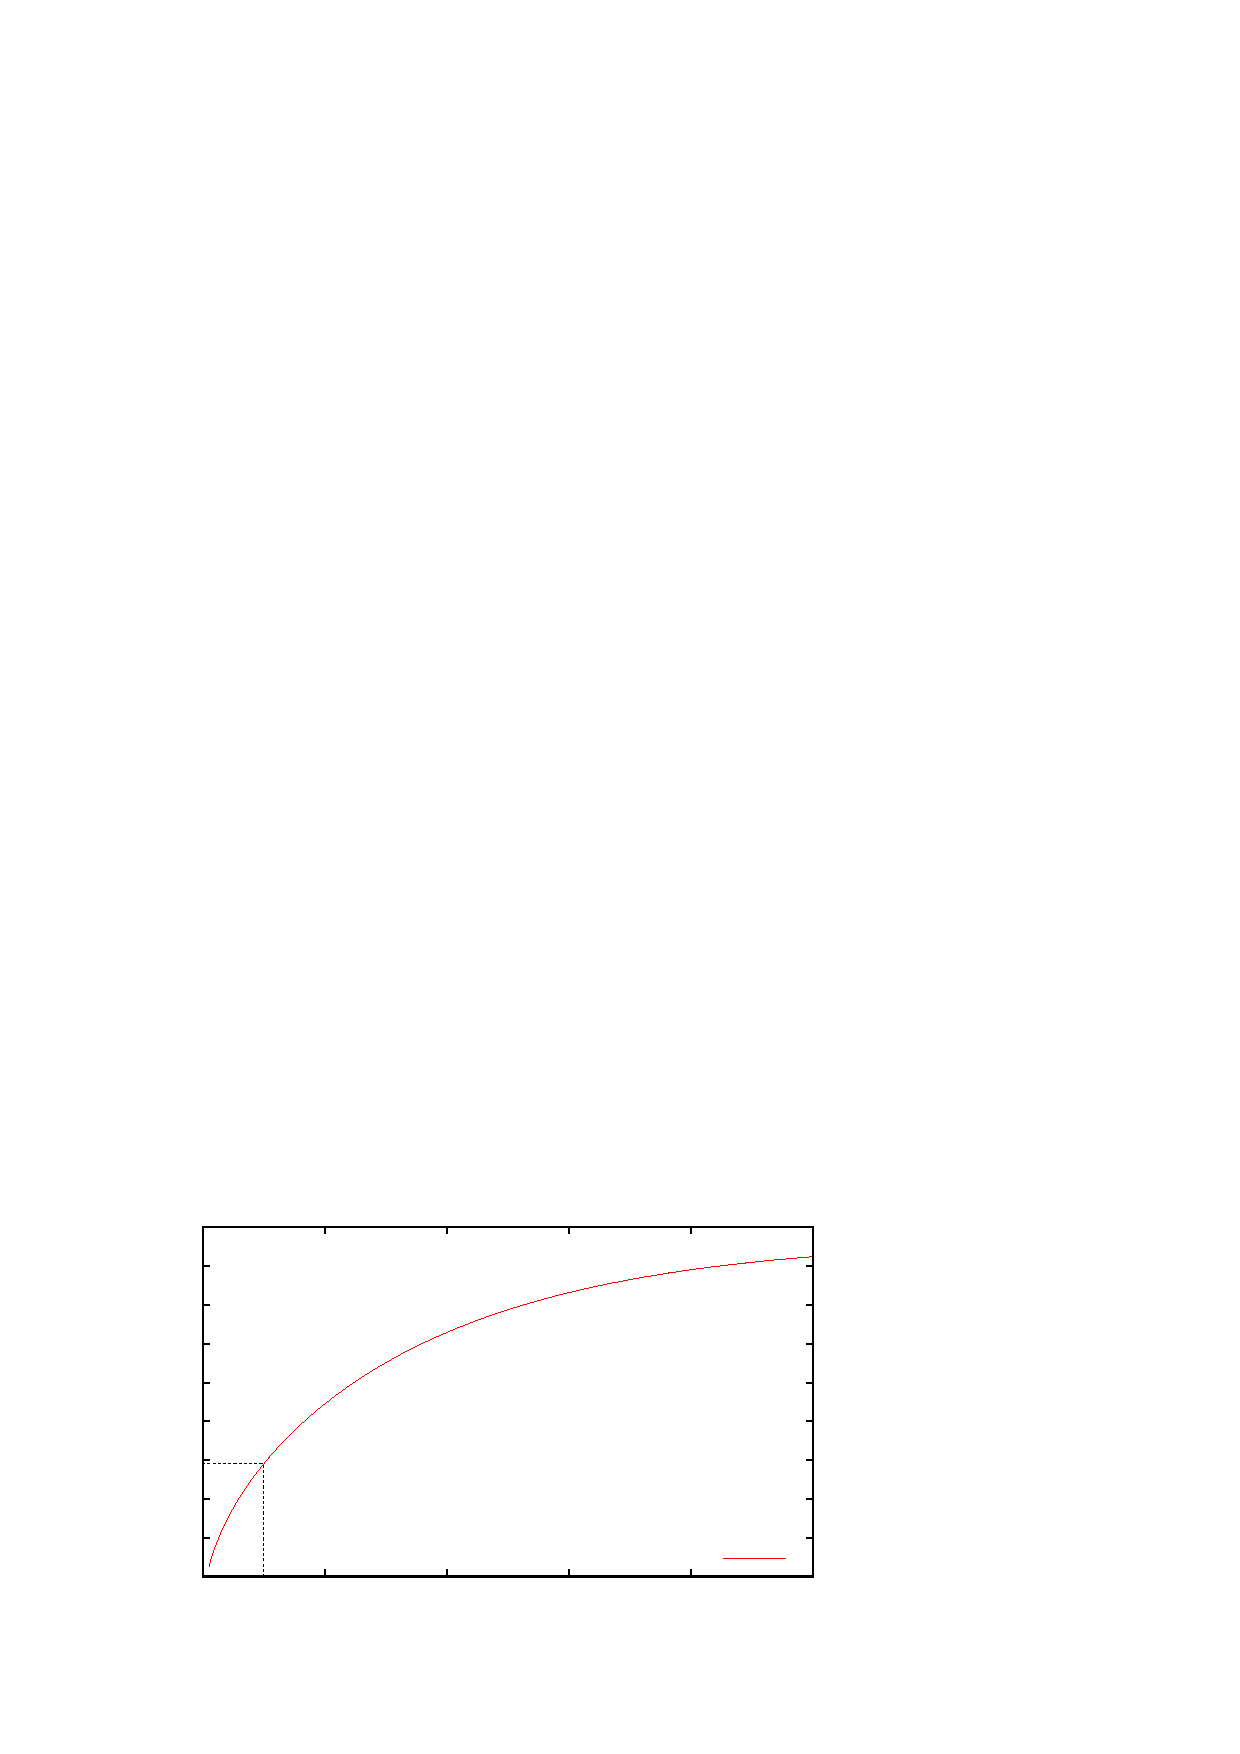
\includegraphics{temperatur}}%
    \gplfronttext
  \end{picture}%
\endgroup

\caption{$T_E$ in Abhängigkeit von $\tilde{n}$}
\label{fig:ergebnisse}
\end{figure}
\noindent In Abbildung \ref{fig:ergebnisse} ist $T_E(\tilde{n})$ grafisch dargestellt (mit Interpolation über 1000 äquidistante Stützstellen). Dort ist ebenfalls der aktuelle Wert ($\tilde{n}=1$) eingezeichnet. Man sieht gut, dass mit steigendem $\tilde{n}$ und damit höherer \ce{CO2}-Konzentration die Temperatur der Erde ein Sättigungsverhalten aufweist; sie steigt immer langsamer. Das Modell ist jedoch nur bedingt gut geeignet, es stellt schon für den Wert von $\tilde{n}=1$ (was dem aktuellen Wert entsprechen würde) eine zu hohe Temperatur dar. 2013 beispielsweise lag die globale Durchschnittstemperatur bei $\num{14.52}\si{\celsius}$ \cite{noaa}. Trotzdem wird qualitativ gut dargestellt, wie sich die Temperatur der Erde mit steigender Anzahl \ce{CO2} Moleküle in der Atmosphäre erhöht.
Die Schwächen des Modells liegen unter anderem darin, dass die Erde kein schwarzer Körper ist, sondern beispielsweise an Wasser und Eis die einfallende Strahlung auch reflektiert. Dies stellt einen Kühleffekt dar, womit die zu hohen Temperaturen des Modells zumindest zum Teil erklärt werden können. Zuletzt muss beachtet werden, dass nur das Treibhausgas \ce{CO2} berücksichtigt wird, obwohl sich die Atmosphäre aus vielen verschiedenen Gasen mit unterschiedlich starken Auswirkungen auf den Treibhauseffekt zusammensetzt (z.B. Wasserdampf, Methan, Ozon).

\begin{thebibliography}{9}

\bibitem{lyness}
 Lyness, J. N.,
 \emph{Notes on the Adaptive Simpson Quadrature Routine},
Journal of the ACM
Volume 16 Issue 3, (1969) 
Seiten 483-495 

\bibitem{noaa}
Global Analysis - Annual 2013, National Climatic Data Center (National Oceanic And Atmospheric Administration) Internet: http://www.ncdc.noaa.gov/sotc/global/2013/13 (2013), abgerufen am 23.05.2014

\end{thebibliography}

\begin{appendix}
\section{Grafiken}

\begin{figure}[htbp!]
\centering
% GNUPLOT: LaTeX picture with Postscript
\begingroup
  \makeatletter
  \providecommand\color[2][]{%
    \GenericError{(gnuplot) \space\space\space\@spaces}{%
      Package color not loaded in conjunction with
      terminal option `colourtext'%
    }{See the gnuplot documentation for explanation.%
    }{Either use 'blacktext' in gnuplot or load the package
      color.sty in LaTeX.}%
    \renewcommand\color[2][]{}%
  }%
  \providecommand\includegraphics[2][]{%
    \GenericError{(gnuplot) \space\space\space\@spaces}{%
      Package graphicx or graphics not loaded%
    }{See the gnuplot documentation for explanation.%
    }{The gnuplot epslatex terminal needs graphicx.sty or graphics.sty.}%
    \renewcommand\includegraphics[2][]{}%
  }%
  \providecommand\rotatebox[2]{#2}%
  \@ifundefined{ifGPcolor}{%
    \newif\ifGPcolor
    \GPcolortrue
  }{}%
  \@ifundefined{ifGPblacktext}{%
    \newif\ifGPblacktext
    \GPblacktextfalse
  }{}%
  % define a \g@addto@macro without @ in the name:
  \let\gplgaddtomacro\g@addto@macro
  % define empty templates for all commands taking text:
  \gdef\gplbacktext{}%
  \gdef\gplfronttext{}%
  \makeatother
  \ifGPblacktext
    % no textcolor at all
    \def\colorrgb#1{}%
    \def\colorgray#1{}%
  \else
    % gray or color?
    \ifGPcolor
      \def\colorrgb#1{\color[rgb]{#1}}%
      \def\colorgray#1{\color[gray]{#1}}%
      \expandafter\def\csname LTw\endcsname{\color{white}}%
      \expandafter\def\csname LTb\endcsname{\color{black}}%
      \expandafter\def\csname LTa\endcsname{\color{black}}%
      \expandafter\def\csname LT0\endcsname{\color[rgb]{1,0,0}}%
      \expandafter\def\csname LT1\endcsname{\color[rgb]{0,1,0}}%
      \expandafter\def\csname LT2\endcsname{\color[rgb]{0,0,1}}%
      \expandafter\def\csname LT3\endcsname{\color[rgb]{1,0,1}}%
      \expandafter\def\csname LT4\endcsname{\color[rgb]{0,1,1}}%
      \expandafter\def\csname LT5\endcsname{\color[rgb]{1,1,0}}%
      \expandafter\def\csname LT6\endcsname{\color[rgb]{0,0,0}}%
      \expandafter\def\csname LT7\endcsname{\color[rgb]{1,0.3,0}}%
      \expandafter\def\csname LT8\endcsname{\color[rgb]{0.5,0.5,0.5}}%
    \else
      % gray
      \def\colorrgb#1{\color{black}}%
      \def\colorgray#1{\color[gray]{#1}}%
      \expandafter\def\csname LTw\endcsname{\color{white}}%
      \expandafter\def\csname LTb\endcsname{\color{black}}%
      \expandafter\def\csname LTa\endcsname{\color{black}}%
      \expandafter\def\csname LT0\endcsname{\color{black}}%
      \expandafter\def\csname LT1\endcsname{\color{black}}%
      \expandafter\def\csname LT2\endcsname{\color{black}}%
      \expandafter\def\csname LT3\endcsname{\color{black}}%
      \expandafter\def\csname LT4\endcsname{\color{black}}%
      \expandafter\def\csname LT5\endcsname{\color{black}}%
      \expandafter\def\csname LT6\endcsname{\color{black}}%
      \expandafter\def\csname LT7\endcsname{\color{black}}%
      \expandafter\def\csname LT8\endcsname{\color{black}}%
    \fi
  \fi
  \setlength{\unitlength}{0.0500bp}%
  \begin{picture}(7200.00,4320.00)%
    \gplgaddtomacro\gplbacktext{%
      \csname LTb\endcsname%
      \put(1474,704){\makebox(0,0)[r]{\strut{} 0}}%
      \put(1474,1374){\makebox(0,0)[r]{\strut{} 5e-20}}%
      \put(1474,2044){\makebox(0,0)[r]{\strut{} 1e-19}}%
      \put(1474,2715){\makebox(0,0)[r]{\strut{} 1.5e-19}}%
      \put(1474,3385){\makebox(0,0)[r]{\strut{} 2e-19}}%
      \put(1474,4055){\makebox(0,0)[r]{\strut{} 2.5e-19}}%
      \put(1606,484){\makebox(0,0){\strut{} 1e+12}}%
      \put(4205,484){\makebox(0,0){\strut{} 1e+13}}%
      \put(6803,484){\makebox(0,0){\strut{} 1e+14}}%
      \put(176,2379){\rotatebox{-270}{\makebox(0,0){\strut{}$\rho(\nu,T=300\si{\Kelvin})(1-f(\nu))$}}}%
      \put(4204,154){\makebox(0,0){\strut{}$\nu$ [\si{\per\second}]}}%
      \put(4204,3945){\makebox(0,0){\strut{}}}%
    }%
    \gplgaddtomacro\gplfronttext{%
      \csname LTb\endcsname%
      \put(2662,3882){\makebox(0,0)[r]{\strut{}$\~n=0.1$}}%
      \csname LTb\endcsname%
      \put(2662,3662){\makebox(0,0)[r]{\strut{}$\~n=1$}}%
      \csname LTb\endcsname%
      \put(2662,3442){\makebox(0,0)[r]{\strut{}$\~n=10$}}%
      \csname LTb\endcsname%
      \put(2662,3222){\makebox(0,0)[r]{\strut{}$\~n=100$}}%
    }%
    \gplbacktext
    \put(0,0){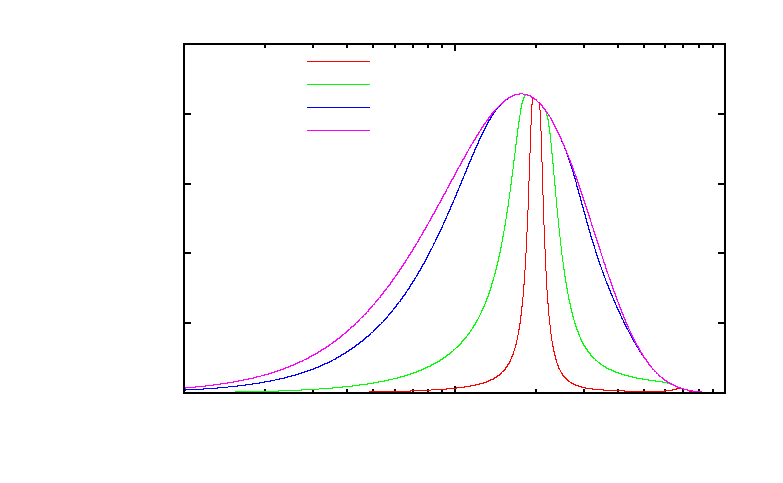
\includegraphics{rho}}%
    \gplfronttext
  \end{picture}%
\endgroup

\caption{Integrand der Emissivität $\epsilon$ für $T=300\, \si{\kelvin}$}
\label{fig:integrand300}
\end{figure}

\begin{figure}[htbp!]
\centering
% GNUPLOT: LaTeX picture with Postscript
\begingroup
  \makeatletter
  \providecommand\color[2][]{%
    \GenericError{(gnuplot) \space\space\space\@spaces}{%
      Package color not loaded in conjunction with
      terminal option `colourtext'%
    }{See the gnuplot documentation for explanation.%
    }{Either use 'blacktext' in gnuplot or load the package
      color.sty in LaTeX.}%
    \renewcommand\color[2][]{}%
  }%
  \providecommand\includegraphics[2][]{%
    \GenericError{(gnuplot) \space\space\space\@spaces}{%
      Package graphicx or graphics not loaded%
    }{See the gnuplot documentation for explanation.%
    }{The gnuplot epslatex terminal needs graphicx.sty or graphics.sty.}%
    \renewcommand\includegraphics[2][]{}%
  }%
  \providecommand\rotatebox[2]{#2}%
  \@ifundefined{ifGPcolor}{%
    \newif\ifGPcolor
    \GPcolortrue
  }{}%
  \@ifundefined{ifGPblacktext}{%
    \newif\ifGPblacktext
    \GPblacktextfalse
  }{}%
  % define a \g@addto@macro without @ in the name:
  \let\gplgaddtomacro\g@addto@macro
  % define empty templates for all commands taking text:
  \gdef\gplbacktext{}%
  \gdef\gplfronttext{}%
  \makeatother
  \ifGPblacktext
    % no textcolor at all
    \def\colorrgb#1{}%
    \def\colorgray#1{}%
  \else
    % gray or color?
    \ifGPcolor
      \def\colorrgb#1{\color[rgb]{#1}}%
      \def\colorgray#1{\color[gray]{#1}}%
      \expandafter\def\csname LTw\endcsname{\color{white}}%
      \expandafter\def\csname LTb\endcsname{\color{black}}%
      \expandafter\def\csname LTa\endcsname{\color{black}}%
      \expandafter\def\csname LT0\endcsname{\color[rgb]{1,0,0}}%
      \expandafter\def\csname LT1\endcsname{\color[rgb]{0,1,0}}%
      \expandafter\def\csname LT2\endcsname{\color[rgb]{0,0,1}}%
      \expandafter\def\csname LT3\endcsname{\color[rgb]{1,0,1}}%
      \expandafter\def\csname LT4\endcsname{\color[rgb]{0,1,1}}%
      \expandafter\def\csname LT5\endcsname{\color[rgb]{1,1,0}}%
      \expandafter\def\csname LT6\endcsname{\color[rgb]{0,0,0}}%
      \expandafter\def\csname LT7\endcsname{\color[rgb]{1,0.3,0}}%
      \expandafter\def\csname LT8\endcsname{\color[rgb]{0.5,0.5,0.5}}%
    \else
      % gray
      \def\colorrgb#1{\color{black}}%
      \def\colorgray#1{\color[gray]{#1}}%
      \expandafter\def\csname LTw\endcsname{\color{white}}%
      \expandafter\def\csname LTb\endcsname{\color{black}}%
      \expandafter\def\csname LTa\endcsname{\color{black}}%
      \expandafter\def\csname LT0\endcsname{\color{black}}%
      \expandafter\def\csname LT1\endcsname{\color{black}}%
      \expandafter\def\csname LT2\endcsname{\color{black}}%
      \expandafter\def\csname LT3\endcsname{\color{black}}%
      \expandafter\def\csname LT4\endcsname{\color{black}}%
      \expandafter\def\csname LT5\endcsname{\color{black}}%
      \expandafter\def\csname LT6\endcsname{\color{black}}%
      \expandafter\def\csname LT7\endcsname{\color{black}}%
      \expandafter\def\csname LT8\endcsname{\color{black}}%
    \fi
  \fi
  \setlength{\unitlength}{0.0500bp}%
  \begin{picture}(7200.00,4320.00)%
    \gplgaddtomacro\gplbacktext{%
      \csname LTb\endcsname%
      \put(1210,704){\makebox(0,0)[r]{\strut{} 0}}%
      \put(1210,1076){\makebox(0,0)[r]{\strut{} 1}}%
      \put(1210,1449){\makebox(0,0)[r]{\strut{} 2}}%
      \put(1210,1821){\makebox(0,0)[r]{\strut{} 3}}%
      \put(1210,2193){\makebox(0,0)[r]{\strut{} 4}}%
      \put(1210,2566){\makebox(0,0)[r]{\strut{} 5}}%
      \put(1210,2938){\makebox(0,0)[r]{\strut{} 6}}%
      \put(1210,3310){\makebox(0,0)[r]{\strut{} 7}}%
      \put(1210,3683){\makebox(0,0)[r]{\strut{} 8}}%
      \put(1210,4055){\makebox(0,0)[r]{\strut{} 9}}%
      \put(1342,484){\makebox(0,0){\strut{} 1e+13}}%
      \put(4073,484){\makebox(0,0){\strut{} 1e+14}}%
      \put(6803,484){\makebox(0,0){\strut{} 1e+15}}%
      \put(176,2379){\rotatebox{-270}{\makebox(0,0){\strut{}$\rho(\nu,T=5750\,\si{\kelvin})(1-f(\nu))$ [$10^{-16}$\,\si{\joule\per\cubic\meter}]}}}%
      \put(4072,154){\makebox(0,0){\strut{}$\nu$ [\si{\per\second}]}}%
      \put(4072,3945){\makebox(0,0){\strut{}}}%
    }%
    \gplgaddtomacro\gplfronttext{%
      \csname LTb\endcsname%
      \put(2398,3882){\makebox(0,0)[r]{\strut{}$\tilde{n}=0.1$}}%
      \csname LTb\endcsname%
      \put(2398,3662){\makebox(0,0)[r]{\strut{}$\tilde{n}=1$}}%
      \csname LTb\endcsname%
      \put(2398,3442){\makebox(0,0)[r]{\strut{}$\tilde{n}=10$}}%
      \csname LTb\endcsname%
      \put(2398,3222){\makebox(0,0)[r]{\strut{}$\tilde{n}=100$}}%
    }%
    \gplbacktext
    \put(0,0){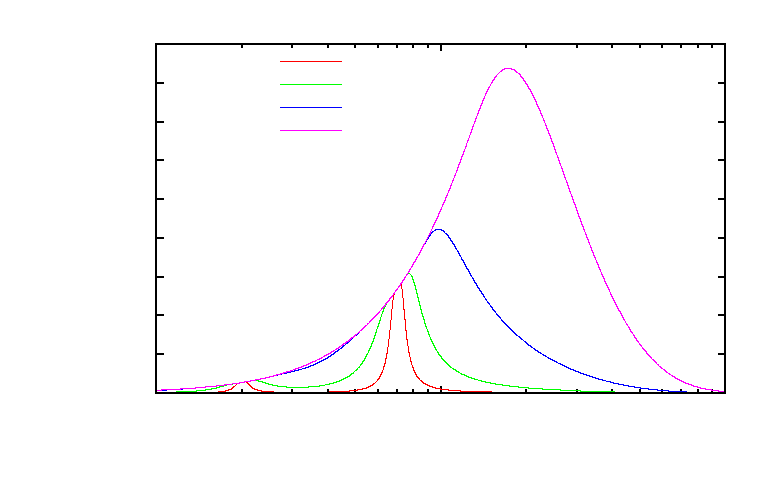
\includegraphics{./figures/rho_sonne}}%
    \gplfronttext
  \end{picture}%
\endgroup

\caption{Integrand der Emissivität $\epsilon$ für $T=5750\, \si{\kelvin}$}
\label{fig:integrand5750}
\end{figure}

\end{appendix}

\end{document}
